% -----------------------------------------------------------------
% Document class: Article
\documentclass[ a4paper, twoside, 11pt]{article}
\usepackage{../../macros-general}
\usepackage{../../macros-article}
% Number of the handout, quiz, exam, etc.
\newcommand{\numero}{01}
\setcounter{numero}{\numero}
\graphicspath{{./figures/}}

% -----------------------------------------------------------------
\begin{document}
\allowdisplaybreaks

% Indices
\newcommand{\iava}{$i$\tsup{ava} }
\newcommand{\iavo}{$i$\tsup{avo} }
\newcommand{\java}{$j$\tsup{ava} }
\newcommand{\javo}{$j$\tsup{avo} }
\newcommand{\kava}{$k$\tsup{ava} }
\newcommand{\kavo}{$k$\tsup{avo} }
\newcommand{\tava}{$t$\tsup{ava} }
\newcommand{\tavo}{$t$\tsup{avo} }
\newcommand{\tmava}{$(t-1)$\tsup{ava} }
\newcommand{\tmavo}{$(t-1)$\tsup{avo} }
\newcommand{\tMava}{$(t+1)$\tsup{ava} }
\newcommand{\tMavo}{$(t+1)$\tsup{avo} }

\begin{center}
\Large Sistemas de Control (EYAG-1005): Tarea \numero \\[1ex]
\small \textbf{Semestre:} 2017-2018 T\'ermino I \qquad
\textbf{Instructor:} Luis I. Reyes Castro
\end{center}
\fullskip

%\fbox{

\begin{minipage}[b][\height][t]{\textwidth}
\vspace{0.2 cm}

\begin{center}
\textbf{COMPROMISO DE HONOR}
\end{center}
\vspace{0.4 cm}

\scriptsize
{
Yo, \rule{60mm}{.1pt} al firmar este compromiso, reconozco que la presente evaluaci\'on est\'a dise\~nada para ser resuelta de manera individual, que puedo usar un l\'apiz o pluma y una calculadora cient\'ifica, \linebreak que solo puedo comunicarme con la persona responsable de la recepci\'on de la evaluaci\'on, y que cualquier instrumento de comunicaci\'on que hubiere tra\'ido debo apagarlo. Tambi\'en estoy conciente que no debo consultar libros, notas, \linebreak ni materiales did\'acticos adicionales a los que el instructor entregue durante la evaluaci\'on o autorice a utilizar. Finalmente, me comprometo a desarrollar y presentar mis respuestas de manera clara y ordenada. \\

Firmo al pie del presente compromiso como constancia de haberlo le\'ido y aceptado. 
\vspace{0.4 cm}

Firma: \rule{60mm}{.1pt} \qquad N\'umero de matr\'icula: \rule{40mm}{.1pt} \hspace{0.5cm} \\[-0.8ex]
}

\end{minipage}

}

\vspace{\baselineskip}



% -----------------------------------------------------------------
\begin{problem}
\textbf{[X Puntos]} En el siguiente sistema mec\'anico la entrada es el torque $T(t)$ y la salida es el desplazamiento del bloque de masa $x(t)$. Encuentre la funci\'on de transferencia, \iec
\[
G(s) \, = \, 
\frac{X(s)}{T(s)}
\]
\begin{figure}[H]
\centering
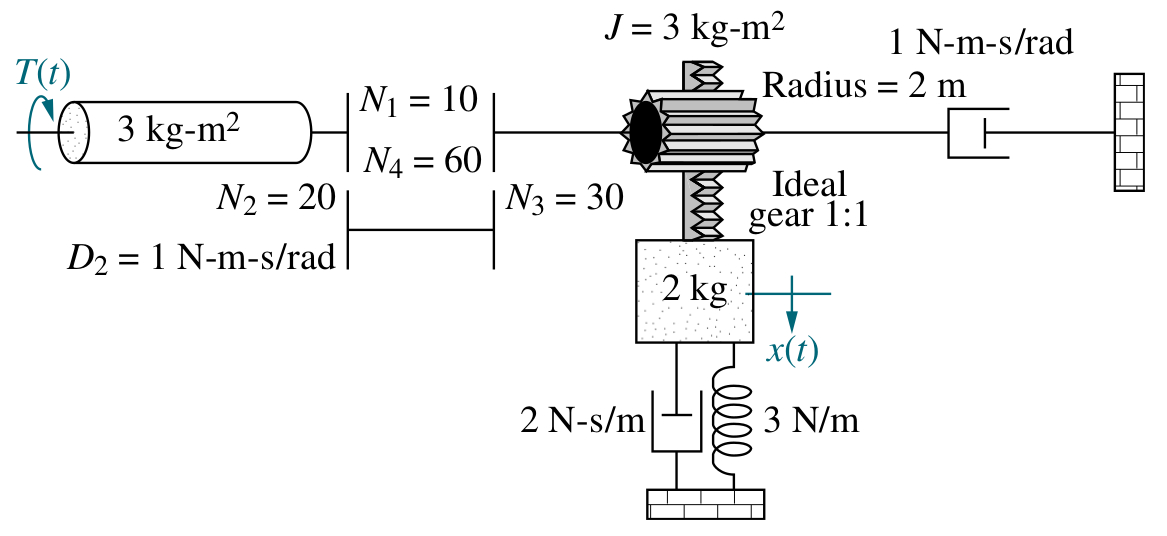
\includegraphics[width=0.68\textwidth]{figures/Nise_Prob-2-40.jpg}
\end{figure}

\end{problem}
\vspace{\baselineskip}

% -----------------------------------------------------------------
\begin{problem}
\textbf{[X Puntos]} En el siguiente sistema mec\'anico la entrada es el torque $T(t)$ y la salida es el desplazamiento del bloque de masa $x(t)$. Encuentre la funci\'on de transferencia, \iec
\[
G(s) \, = \, 
\frac{X(s)}{T(s)}
\]
\begin{figure}[H]
\centering
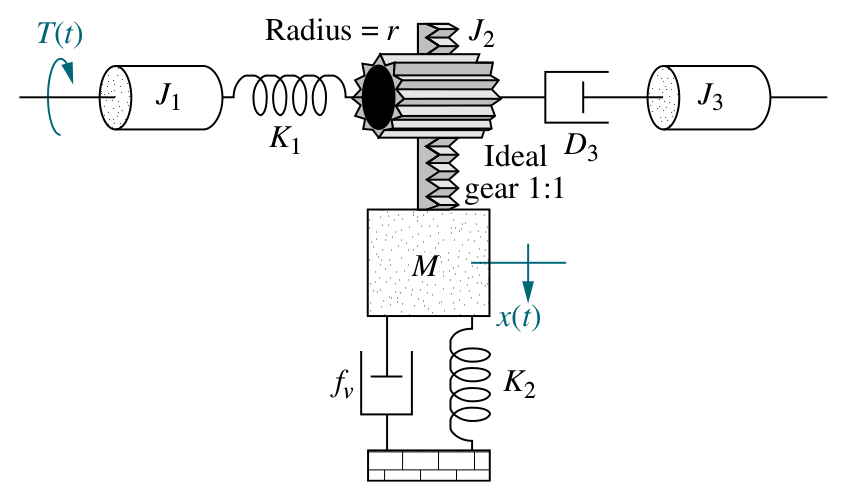
\includegraphics[width=0.6\textwidth]{figures/Nise_Prob-2-41.jpg}
\end{figure}

\end{problem}
\vspace{\baselineskip}


% -----------------------------------------------------------------
\begin{problem}
\textbf{[X Puntos]} Considere el siguiente sistema mec\'anico donde un motor DC controlado por armadura sirve de actuador. La entrada es el voltage de la armadura $e_a(t)$ y la salida es el desplazamiento angular $\theta_2(t)$. Encuentre la funci\'on de transferencia, \iec
\[
G(s) \, = \, 
\frac{\Theta_2(s)}{E_a(s)}
\]
\begin{figure}[H]
\centering
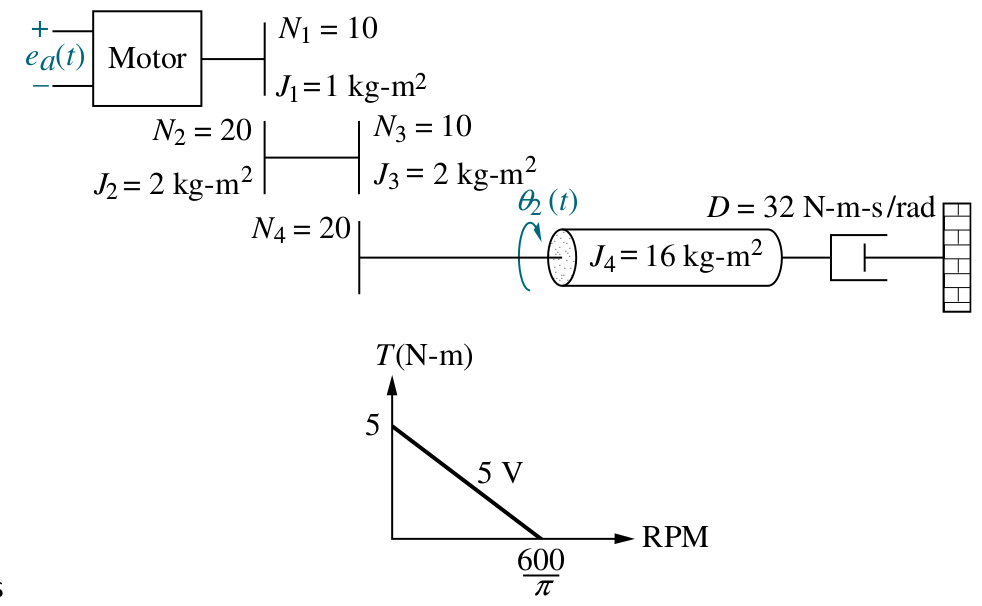
\includegraphics[width=0.66\textwidth]{figures/Nise_Prob-2-43.jpg}
\end{figure}

\end{problem}
\vspace{\baselineskip}

%% -----------------------------------------------------------------
%\begin{problem}
%\textbf{[X Puntos]} Considere el siguiente sistema mec\'anico donde un motor DC controlado por armadura sirve de actuador. La entrada es el voltage de la armadura $e_a(t)$ y la salida es el desplazamiento $x(t)$. Encuentre la funci\'on de transferencia, \iec
%\[
%G(s) \, = \, 
%\frac{X(s)}{E_a(s)}
%\]
%\begin{figure}[H]
%\centering
%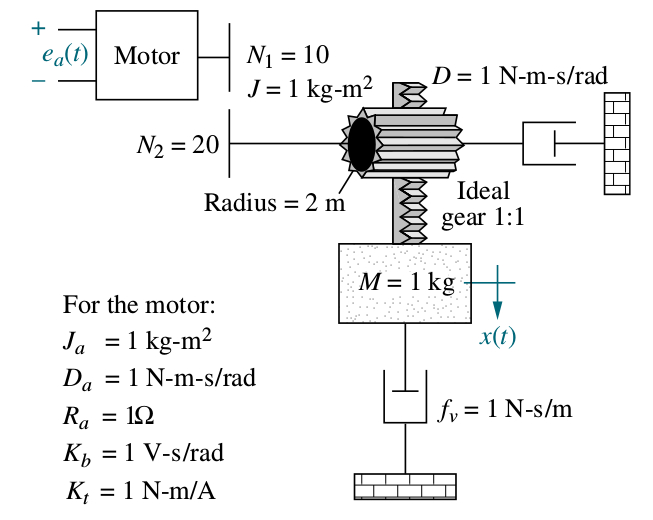
\includegraphics[width=0.54\textwidth]{figures/Nise_Prob-2-46.jpg}
%\end{figure}
%
%\end{problem}
%\vspace{\baselineskip}

% -----------------------------------------------------------------
\begin{problem}
\textbf{[X Puntos]} Considere el siguiente modelo de un giroscopio, donde la ecuaci\'on diferencial se muestra arriba del esquema del sistema. Escriba la funci\'on de transferencia, \iec
\[
G(s) \, = \, 
\frac{\Theta_x(s)}{\Theta_z(s)}
\]

\begin{figure}[H]
\centering
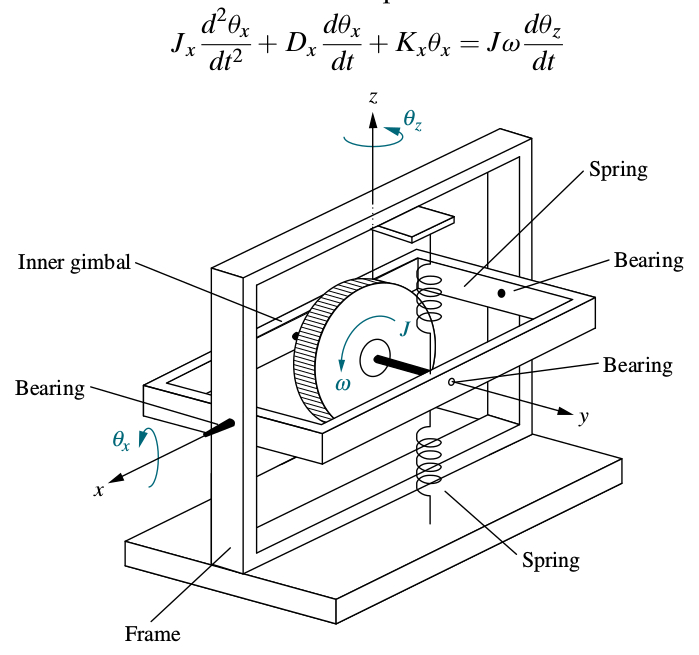
\includegraphics[width=0.6\textwidth]{figures/Nise_Prob-3-17.jpg}
\end{figure}

\end{problem}
\vspace{\baselineskip}

% -----------------------------------------------------------------
\begin{problem}
\textbf{[X Puntos]} Para el siguiente sistema de control, encuentre su funci\'on de transferencia en circuito cerrado como funci\'on de $K$. 

\begin{figure}[H]
\centering
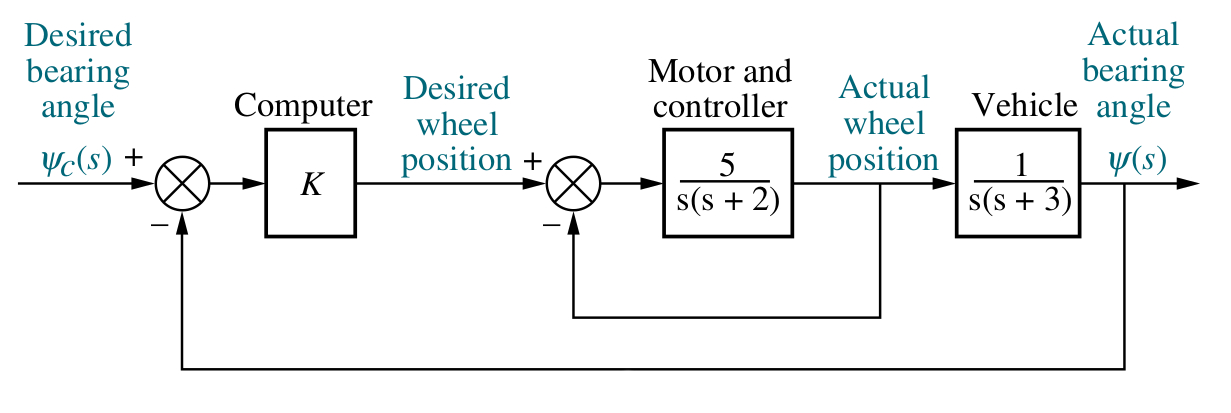
\includegraphics[width=0.8\textwidth]{figures/Nise_Prob-5-51.jpg}
\end{figure}

\end{problem}
\vspace{\baselineskip}

\end{document}
